
	% filters
\subsection{Filters}

\begin{frame} % -------------------------------------------------------------
	\frametitle{Filters}
	\begin{itemize}
		\item general \textbf{filter types}:
			\begin{itemize}
				\item \textbf{low-pass}: passes low frequencies (cuts high ones)
				\item \textbf{high-pass}: passes high frequencies (cuts low ones)
				\item \textbf{band-pass}: passes a range of frequencies (combination of low- and high-pass)
				\item \textbf{band-stop} (notch): cuts a range of frequencies (opposite of band-pass)
			\end{itemize}
		\item \textbf{cutoff frequency} at which output power is (generally) reduced by $-3\,\textrm{dB}$
		\item \textbf{example}: \texttt{matlab/filters.m}
			\begin{figure}
				\centering
				\begin{subfigure}[c]{0.48\linewidth}
					\cfbox{neutral}{\includegraphics[width=\linewidth]{images/filters_high.eps}}
				\end{subfigure}
				\hspace{0.01\linewidth}
				\begin{subfigure}[c]{0.48\linewidth}
					\cfbox{neutral}{\includegraphics[width=\linewidth]{images/filters_low.eps}}
				\end{subfigure}
			\end{figure}
	\end{itemize}
\end{frame}

\begin{frame} % -------------------------------------------------------------
	\frametitle{Filters}
	\begin{itemize}
		\item many \textbf{filter families} with different characteristics (\texttt{matlab/filters2.m}), e.\,g.
			\begin{figure}
				\centering
				\begin{subfigure}[c]{0.8\linewidth}
					\cfbox{neutral}{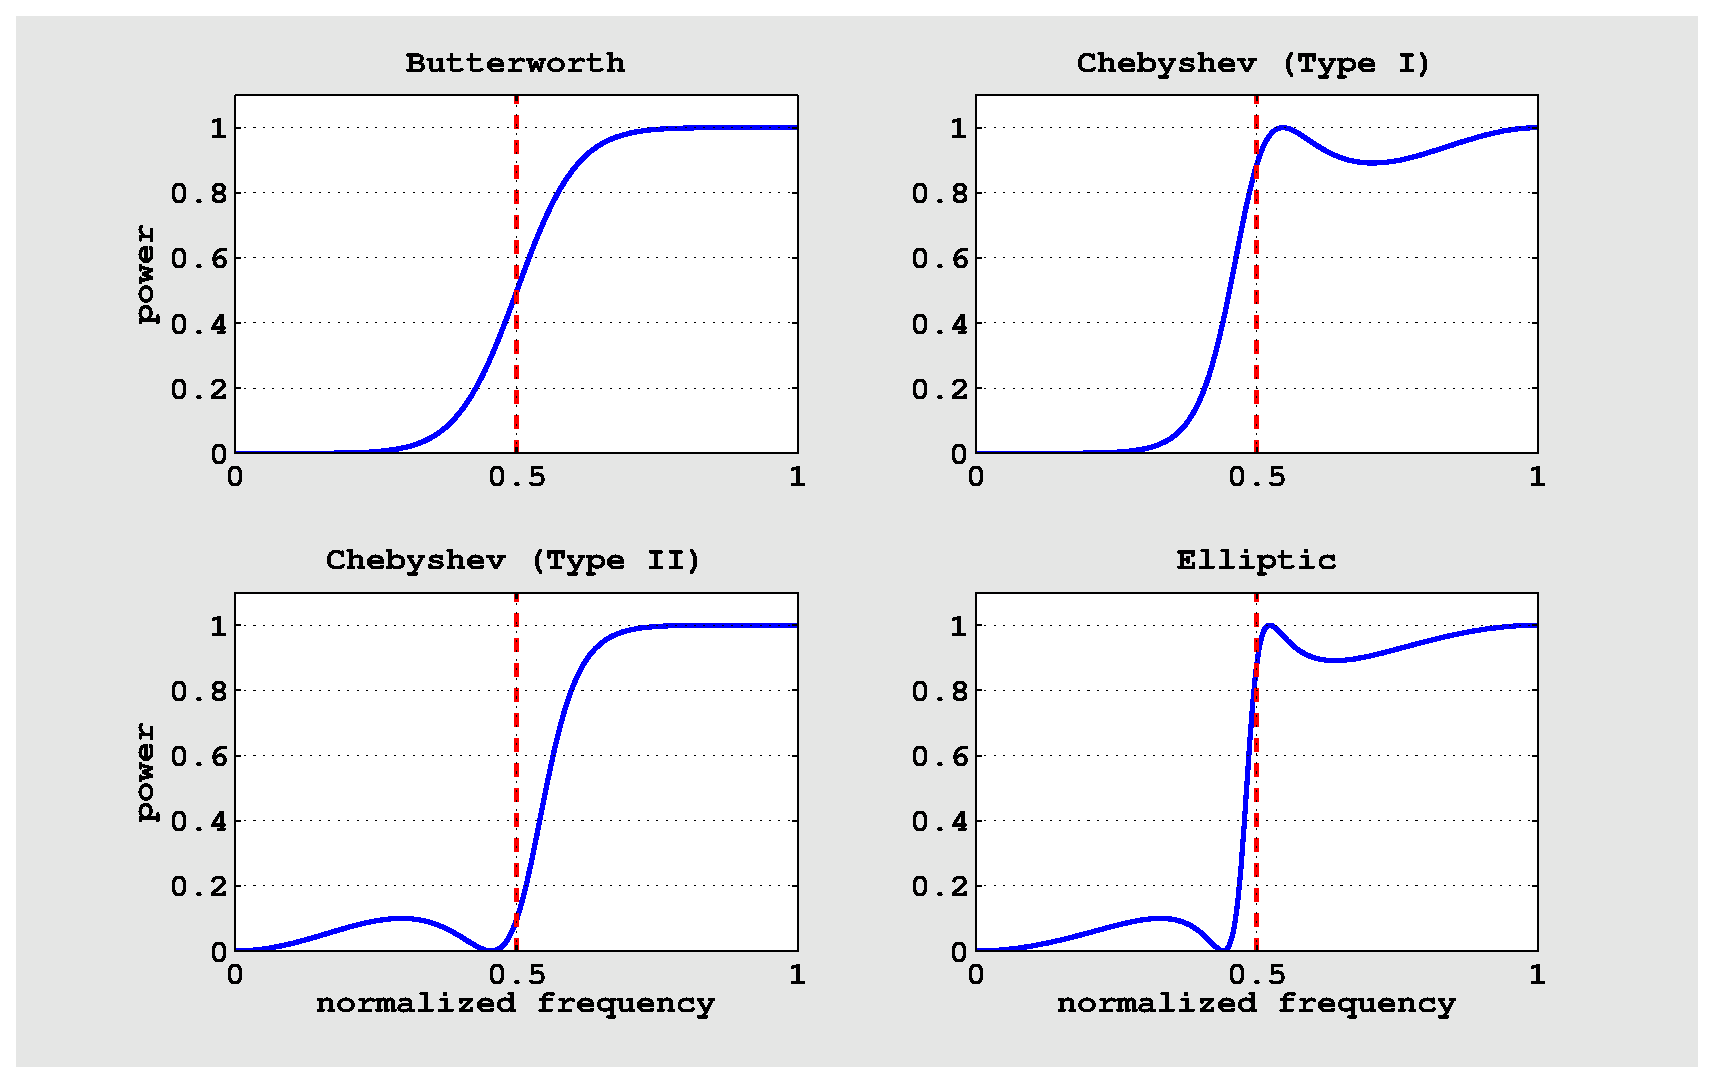
\includegraphics[width=0.9\linewidth]{images/filters.eps}}
				\end{subfigure}
			\end{figure}
		\item \textbf{normalized frequency}
			\begin{align*}
				\tilde f_k=\frac{f_k}{f_{\textrm{Ny}}}=\frac{2f_k}{f_{\textrm S}}\in[0,1]\quad\textrm{with}\quad k\in\{1,\ldots,N\}
			\end{align*}
	\end{itemize}
\end{frame}

\begin{frame} % -------------------------------------------------------------
	\frametitle{Filters}
	\begin{itemize}
		\item filters are represented by \textbf{filter coefficients} $b_j$ (feedforward) and $a_j$ (feedback)
		\item high \textbf{filter order} $m$ increases computational complexity but thereby quality
			\begin{align*}
				y_i=\overbrace{\frac1{a_1}\Bigg(\underbrace{\sum_{j=0}^mb_{j+1}x_{i-j}}_{\textrm{FIR}}-\sum_{j=1}^ma_{j+1}y_{i-j}\Bigg)}^{\textrm{IIR}}\quad\textrm{with}\quad i\in\{1,\ldots,N\}
			\end{align*}
		\item \textbf{FIR filters} (finite impulse response) are slow to compute but stable
		\item \textbf{IIR filters} (infinite impulse response) are fast to compute but might be unstable
		\item some often used \textbf{additional terms} (images from \url{http://dspguru.com})
			\begin{figure}
				\centering
				\begin{subfigure}[c]{0.48\linewidth}
					\cfbox{neutral}{\includegraphics[width=0.9\linewidth]{images/response.png}}
				\end{subfigure}
				\hspace{0.01\linewidth}
				\begin{subfigure}[c]{0.48\linewidth}
					\cfbox{neutral}{\includegraphics[width=0.9\linewidth]{images/ripple.png}}
				\end{subfigure}
			\end{figure}
	\end{itemize}
\end{frame}

\begin{frame}[fragile] % ----------------------------------------------------
	\frametitle{Filters}
	\begin{itemize}
		\item \textbf{Butterworth filter} (high-pass, second-order, $100\,\textrm{Hz}$ cutoff)
			\begin{code}
>> m = 2; \color{medium}% filter order
>> cutoff = 100; \color{medium}% cutoff frequency
>> [b, a] = butter( m, cutoff / (fS/2), 'high' );
			\end{code}
		\item \textbf{Chebyshev filter} (high-pass, $1\,\textrm{dB}$ ripple, $40\,\textrm{dB}$ attenuation, $100\,\textrm{Hz}$ cutoff)
			\begin{code}
>> cutoff = 100; \color{medium}% cutoff frequency
>> stopband = 90; \color{medium}% stopband frequency
>> ripple = 1; \color{medium}% passband ripple
>> attenuation = 40; \color{medium}% stopband attenuation
>> m = cheb2ord( cutoff / (fS/2), stopband / (fS/2), ripple, attenuation );
>> [b, a] = cheby2( m, attenuation, stopband / (fS/2) );
			\end{code}
		\item \textbf{apply any filter}
			\begin{code}
>> y = filter( b, a, x ); \color{medium}% filter signal x using coefficients a, b
			\end{code}
		\item or in zero-phase version (without filter delay)
			\begin{code}
>> y = filtfilt( b, a, x ); \color{medium}% zero-phase filtering
			\end{code}
		%\item plot filter response
			%\begin{code}
%>> [h, f] = freqz( b, a, 512, fS ); \color{medium}% complex filter response
%>> plot( f, abs( h ).^2 );
			%\end{code}
	\end{itemize}
\end{frame}

\begin{frame} % -------------------------------------------------------------
	\frametitle{Filters}
	\begin{itemize}
		\item \textbf{exercise}:
			\begin{itemize}
				\item Can you image what \textbf{filter delay} means?
				\item TODO: home audio/hifi, bass and treble
			\end{itemize}
	\end{itemize}
\end{frame}

